% Bagean: sajarah
% Bab: téori himpunan
% Pérangan: limit

\documentclass[../../../include/open-logic-section]{subfiles}

\begin{document}
	
\olfileid{his}{set}{limits}	

\olsection{Dhéfinisi Limit kang Ketat}
	
Ing jaman saiki, cara baku ngrampungaké masalah
kang lagi dirembug yaiku nyingkirké
infinitesimal. Mangkéné carané.

Kita wis weruh yèn nalika $\beta$ saya cilik,
taksiran gradiené saya becik. Malah, nalika
$\beta$ bisa saya cedhak marang $0$ tanpa
wates, taksiran kanggo $f'(c)$ ``saya
nyedhaki'' gradien kang dikarepaké.
Mula, tinimbang nimbang apa kang kelakon
\emph{ing} $\beta = 0$, kita mung perlu
nimbang \emph{arah owahé} taksiran
kanggo $f'(c)$ nalika $\beta$
nyedhaki $0$.

Kanthi cara ngandharaké iki, tantangan
umumé yaiku menehi teges marang
pratelan kang awujud mangkéné:
\begin{center}
Nalika $x$ nyedhaki $c$, $g(x)$ saya nyedhaki $\ell$.
\end{center}
kang bisa ditulis luwih cekak mangkéné:
\[
\lim_{x \rightarrow c}g(x) = \ell.
\]
Ing abad kaping sangalas, kanthi nerusaké
karya Cauchy, Weierstrass maringi dhéfinisi
kang ketat kanggo ekspresi iki. Gagasané
yaiku kita bisa nggawé $g(x)$ sacedhak
kang dikarepaké karo~$\ell$, kanthi
nggawé $x$ cukup cedhak karo~$c$.
Luwih persis, kita netepaké yèn
$\lim_{x \rightarrow c} g(x) = \ell$
ateges:
\[
(\forall\epsilon > 0)(\exists \delta > 0)\forall x \left(0 < |x - c| < \delta \lif |g(x) - \ell| < \epsilon \right).
\]
Garis-garis tegak ing kéné nandhani
nilai mutlak. Tegesé, $|x| = x$
yèn $x \geq 0$, lan $|x| =-x$
yèn $x < 0$; fungsi \emph{iku}
bisa digambar mangkéné:
\begin{center}
	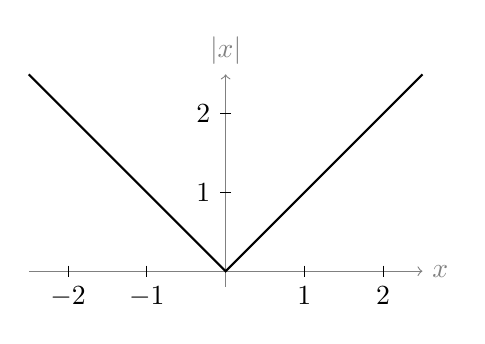
\begin{tikzpicture}[scale=1]
	\draw[->, gray] (-2.5,0) -- (2.5,0) node[right] {$x$};
	\draw[->, gray] (0,-.2) -- (0,2.5) node[above] {$|x|$};
	
	\foreach \x/\xtext in {-2/-2, -1/-1, 1/1, 2/2}
	\draw[shift={(\x,0)}] (0pt,2pt) -- (0pt,-2pt) node[below] {{$\xtext$}};
	
	\foreach \y/\ytext in {1/1, 2/2}
	\draw[shift={(0,\y)}] (2pt,0pt) -- (-2pt,0pt) node[left] {{$\ytext$}};
	
	\draw[thick] (-2.5, 2.5)--(0,0)--(2.5, 2.5);
	\end{tikzpicture}
\end{center}
Dadi, kanthi kasar, dhéfinisi iki
nyatakaké: ``kaluputan'' bisa digawe
kurang saka $\epsilon$ (yaiku,
$|g(x) - \ell| < \epsilon$) kanthi
milih argumèn kang ora padha
karo c lan jaraké kurang saka
$\delta$ saka~$c$ (yaiku,
$0 < |x - c| < \delta$).

Sawisé ndhéfinisikaké limit,
kita bisa ngindhari infinitesimal
babar pisan, kanthi netepaké
yèn gradien $f$ ing $c$
diwènèhaké déning:
\[
	{f}'(c) = \lim_{x \rightarrow 0}\left(\frac{f(c +x) - f(c)}{x}\right) \text{ yèn limité ana}.
\]
Nanging kudu dimangertèni sebabé
dhéfinisi iki mbutuhaké syarat
``yèn limité ana''. Upamané,
delengen $f(x) = |x|$, kang
grafiké mau wis kita deleng.
Cetha yèn $f'(0)$ ora
didhéfinisikaké kanthi becik:
yèn kita nyedhaki $0$
``saka tengen'', gradiené
tansah $1$; yèn kita
nyedhaki $0$ ``saka kiwa'',
gradiené tansah $-1$;
mula limité ora ana.
Mula kita bisa nambahaké:
fungsi~$f$ iku
\emph{bisa didiferensiasi}
ing~$x$ yèn lan mung yèn
limit kaya iku ana.

Kita wis weruh cara nggarap diferensiasi
nganggo gagasan \emph{limit}.
Gagasan kang padha bisa dienggo
ndhéfinisikaké fungsi kang
\emph{kontinu}. (Bolzano sakjané
wis mangertèni bab iki ing taun
1817.) Andharan Cauchy--Weierstrass
ngenani kontinuitas mangkéné.
Kanthi kasar: fungsi~$f$ kontinu
(ing sawijining titik) yèn
kita bisa njamin tingkat katliten
kang dikarepaké ing output
fungsi kanthi njaluk tingkat katliten
tartamtu ing inputé. Luwih
persis: $f$ kontinu ing $c$
yèn, nalika $x$ nyedhaki
nol, béda antarane $f(c + x)$
lan $f(c)$ uga nyedhaki $0$.
Tegesé, $f$ \emph{kontinu}
ing $c$ yèn lan mung yèn
$f(c) = \lim_{x \rightarrow c} f(x)$.

Yèn diterusaké, kita bakal mlebu
analisis real, déné topik kita
iku téori himpunan. Mula saiki
kita mandheg sedhéla kanggo
nyebut piwulangé. Sajroning
abad kaping sangalas,
para matématikawan sinau
nggarap tanpa infinitesimal,
kanthi migunakaké gagasan
\emph{limit} kang didhéfinisikaké
kanthi ketat.

\end{document}
